\newpage
\subsection{Caso d'uso UC2: Main post-autenticazione }
\label{UC2}
\begin{figure}[ht]
	\centering
	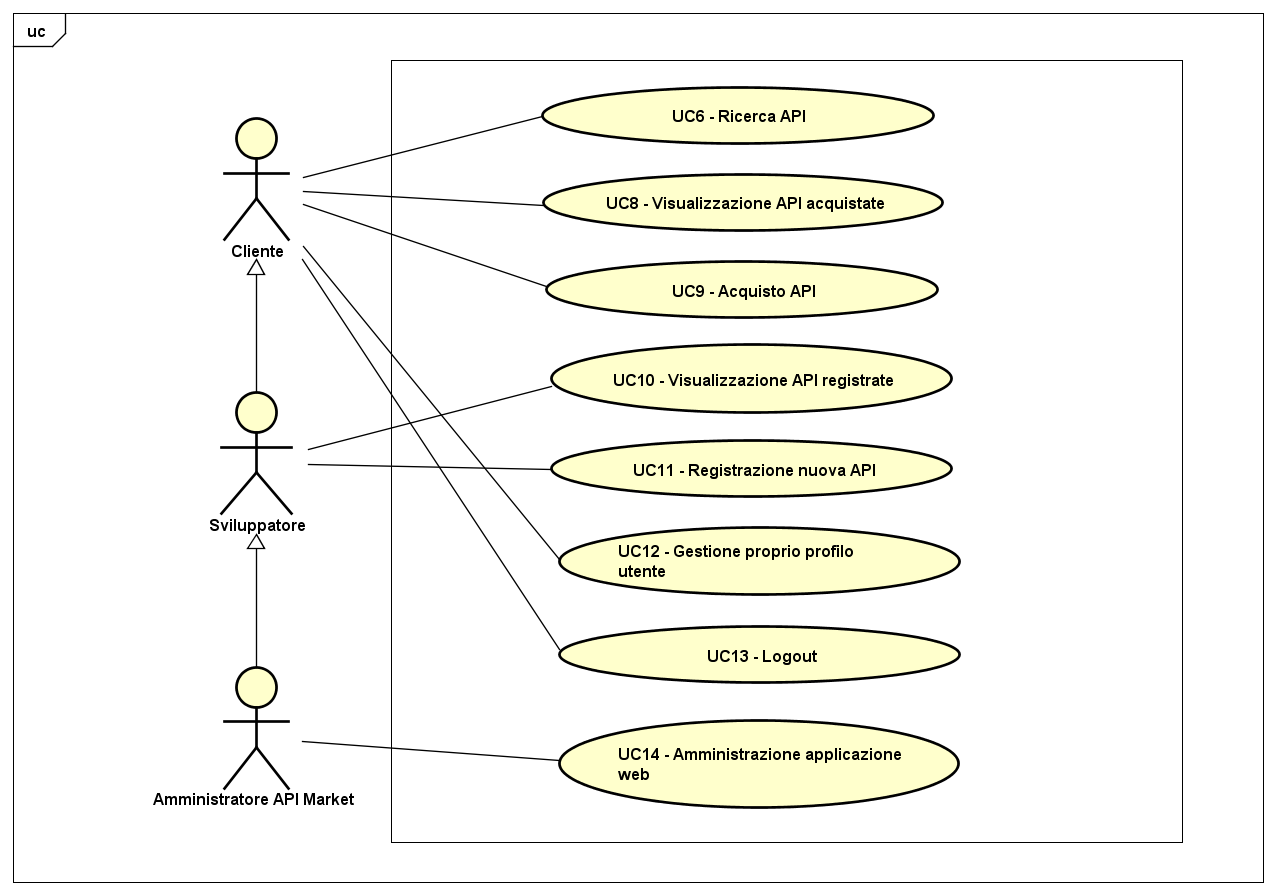
\includegraphics[scale=0.45]{UML/UC2.png}
	\caption{UC2: Main post-autenticazione}
\end{figure}

\begin{longtable}{ l | p{11cm}}
	\hline
	\rowcolor{Gray}
	 \multicolumn{2}{c}{UC2 - Main post-autenticazione} \\
	 \hline
	\textbf{Attori} & Cliente, Sviluppatore, Amministratore API Market \\
	\textbf{Descrizione} & L'attore tramite la schermata principale
	dell'applicazione, può accedere e sfruttare le funzionalità a lui disponibili: la ricerca API, la visualizzazione di API acquistate, l'acquisto API, la gestione del proprio profilo utente, il logout.
	Lo sviluppatore, oltre alle funzionalità offerte all'utente autenticato, può visualizzare le API registrate e registrarne di nuove.
	L'amministratore API Market, oltre alle funzionalità offerte all'utente autenticato, può amministrare l'applicazione web. \\
	\textbf{Pre-Condizioni} & L'attore ha avviato l'applicazione web e si è autenticato \\
	\textbf{Post-Condizioni} & L'applicazione ha eseguito le richieste dell'attore \\
	\textbf{Scenario Principale} & 
	\begin{enumerate*}[label=(\arabic*.),itemjoin={\newline}]
		\item L'attore può effettuare una ricerca sulle API presenti nell'applicazione
(UC6)
		\item L'attore può visualizzare le API da lui acquistate (UC8)
		\item L'attore può acquistare una API (UC9)
		\item Lo sviluppatore può visualizzare le API da lui registrate (UC10)
		\item Lo sviluppatore può registrare una nuova API (UC11)
		\item L'attore può gestire il proprio profilo utente (UC12)
		\item L'attore può effettuare il logout (UC13)
		\item L'amministratore API Market può accedere all'amministrazione dell'applicazione web (UC14)
	\end{enumerate*}\\
\end{longtable}